\documentclass[12pt]{article}
\usepackage[papersize={8cm,12cm},margin={.5cm,.5cm}]{geometry}
\usepackage{common}
\usepackage{amssymb}
\begin{document}
\begin{problem}
\item[7.] $\triangle{ABC}$ 中,$D$、$E$ 兩點分別在 $\overline{AB}$、$\overline{BC}$ 上,如圖(七)所示。若 $\overline{AD}:\overline{DB} = \overline{CE}:\overline{EB} = 2:3$,則 $\triangle{BDE}$ 與 $\triangle{ADC}$ 的面積比為何?
  \begin{figure}[ht]
    \centering
    \vspace*{-1ex}
    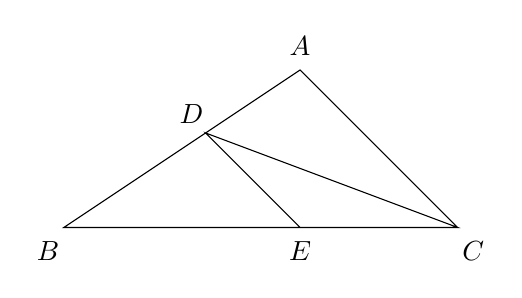
\begin{tikzpicture}
      \draw (5,0) -- (3,2) -- (0,0) -- (5,0) -- (1.8,1.2) -- (3,0);
      \node at (3,2.3) {$A$};
      \node at (-.2,-.3) {$B$};
      \node at (5.2,-.3) {$C$};
      \node at (1.62,1.44) {$D$};
      \node at (3,-.3) {$E$};
    \end{tikzpicture}
    \vspace*{-1ex}
    \caption*{圖(七)}
    \vspace*{-2ex}
  \end{figure}
  \begin{choices}
    \item $3:5$
    \item $4:5$
    \item $9:10$
    \item $15:16$
  \end{choices}
\end{problem}
\end{document}
